Plots are normalized to 1$/fb$. 
Error bars are the sum in quadrature of the statistical uncertainty of EPS and post-EPS data. 
EPS dataset corresponds to run$<$170826, post-EPS to run$\geq$170826.

\clearpage

\begin{figure}[!hbtp]
\centering
\subfigure[]{
\centering
\label{subfig:lp_dPhi_ww0j}
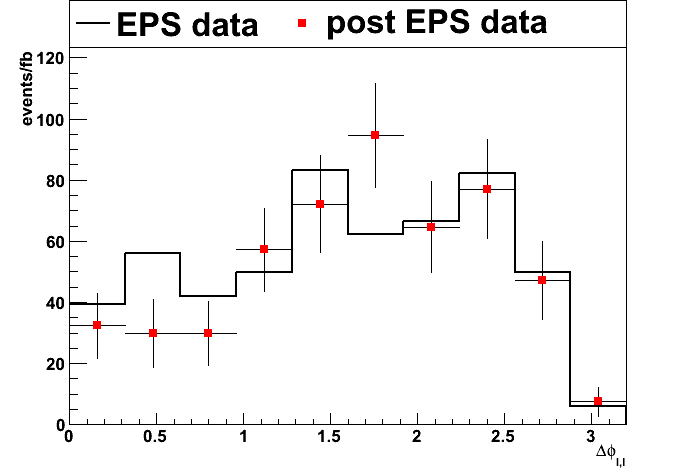
\includegraphics[width=.32\textwidth]{lp_figures/postEPSvalid/hm0/dPhi_ww0j.png}}
\subfigure[]{
\centering
\label{subfig:lp_dilepmass_ww0j}
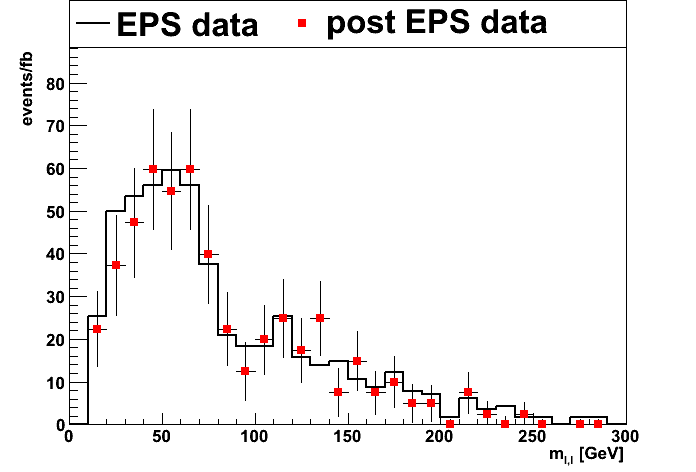
\includegraphics[width=.32\textwidth]{lp_figures/postEPSvalid/hm0/dilepmass_ww0j.png}}\\
\subfigure[]{
\centering
\label{subfig:lp_dileppt_ww0j}
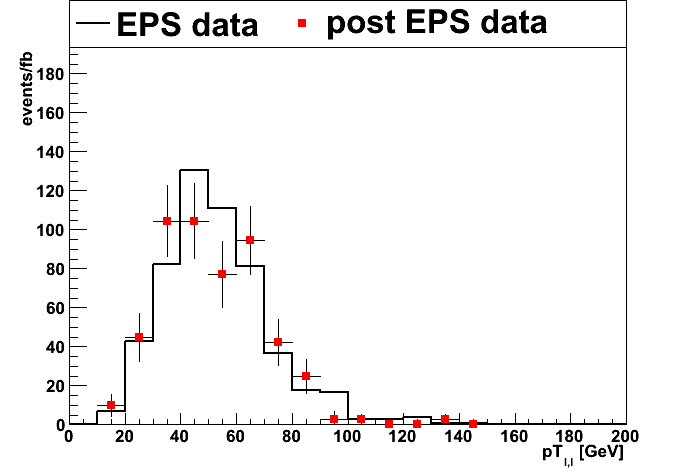
\includegraphics[width=.32\textwidth]{lp_figures/postEPSvalid/hm0/dileppt_ww0j.png}}
\subfigure[]{
\centering
\label{subfig:lp_type_ww0j}
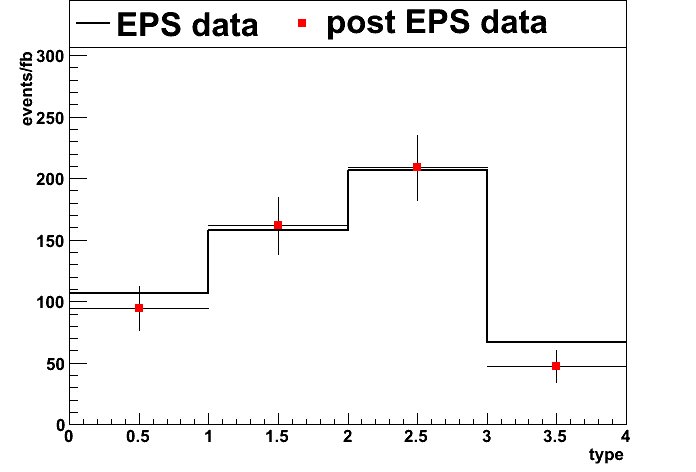
\includegraphics[width=.32\textwidth]{lp_figures/postEPSvalid/hm0/type_ww0j.png}}
\caption{EPS and post-EPS data comparison: 0-jet bin, all final states. 
\subref{subfig:lp_dPhi_ww0j} $\Delta\phi$ between the two leptons;
\subref{subfig:lp_dilepmass_ww0j} di-lepton invariant mass;
\subref{subfig:lp_dileppt_ww0j} di-lepton transverse momentum;
\subref{subfig:lp_type_ww0j} di-lepton type ($\mu\mu$=0, $\mu e$=2, $e\mu$=2, $ee$=3).
}
\label{fig:lp_ww0j_dilep}
\end{figure}

\begin{figure}[!hbtp]
\centering
\subfigure[]{
\centering
\label{subfig:lp_lep1pt_ww0j}
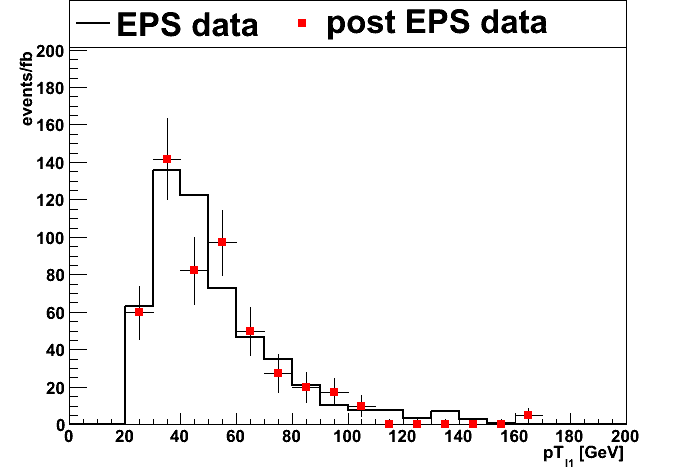
\includegraphics[width=.32\textwidth]{lp_figures/postEPSvalid/hm0/lep1pt_ww0j.png}}
\subfigure[]{
\centering
\label{subfig:lp_lep2pt_ww0j}
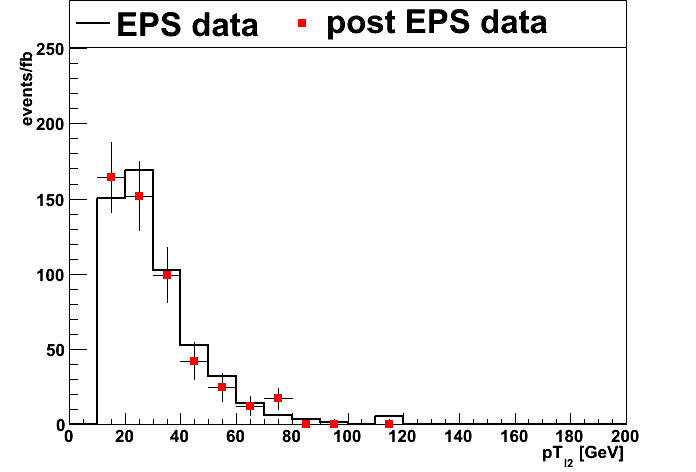
\includegraphics[width=.32\textwidth]{lp_figures/postEPSvalid/hm0/lep2pt_ww0j.png}}
\subfigure[]{
\centering
\label{subfig:lp_jet1pt_ww0j}
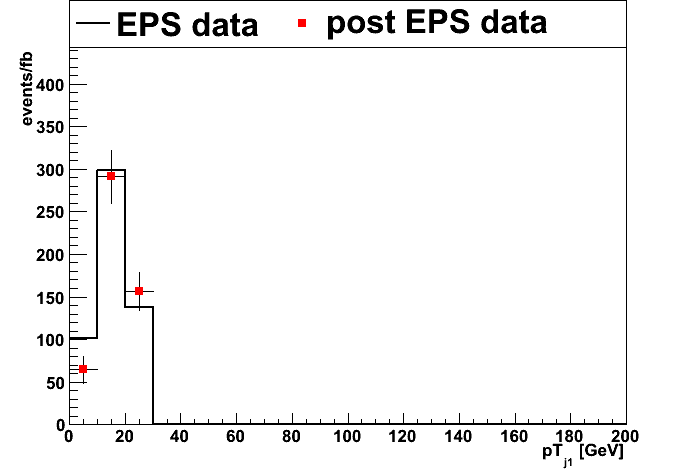
\includegraphics[width=.32\textwidth]{lp_figures/postEPSvalid/hm0/jet1pt_ww0j.png}}\\
\subfigure[]{
\centering
\label{subfig:lp_pmet_ww0j}
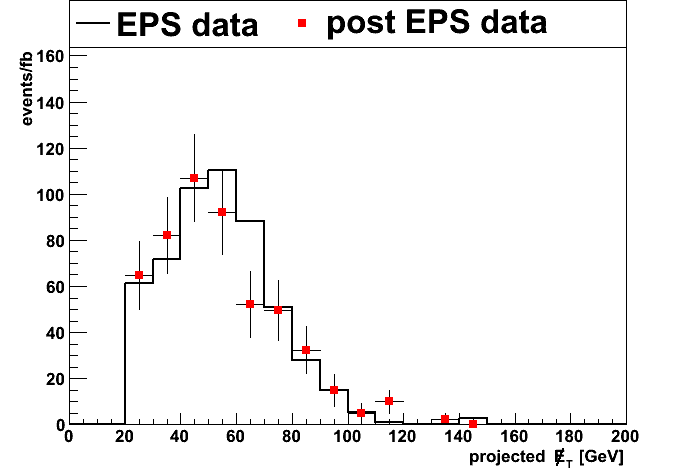
\includegraphics[width=.32\textwidth]{lp_figures/postEPSvalid/hm0/pmet_ww0j.png}}
\subfigure[]{
\centering
\label{subfig:lp_pTrackMet_ww0j}
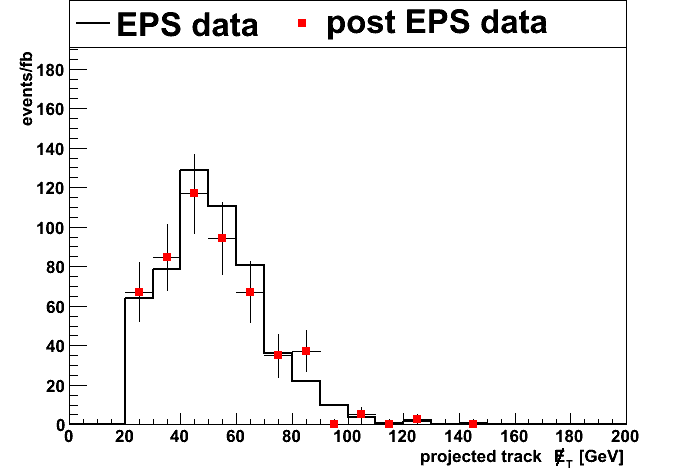
\includegraphics[width=.32\textwidth]{lp_figures/postEPSvalid/hm0/pTrackMet_ww0j.png}}
\subfigure[]{
\centering
\label{subfig:lp_mt_ww0j}
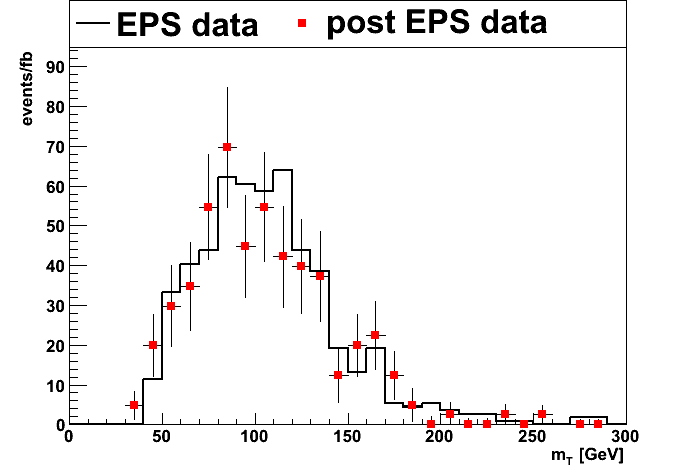
\includegraphics[width=.32\textwidth]{lp_figures/postEPSvalid/hm0/mt_ww0j.png}}
\caption{EPS and post-EPS data comparison: 0-jet bin, all final states. 
\subref{subfig:lp_lep1pt_ww0j} leading lepton $p_T$;
\subref{subfig:lp_lep2pt_ww0j} trailing lepton $p_T$;
\subref{subfig:lp_jet1pt_ww0j} leading jet $p_T$;
\subref{subfig:lp_pmet_ww0j} projected MET;
\subref{subfig:lp_pTrackMet_ww0j} projected track-MET;
\subref{subfig:lp_mt_ww0j} transverse mass of dilepton-MET system.
}
\label{fig:lp_ww0j_lepjetmet}
\end{figure}

\clearpage

\begin{figure}[!hbtp]
\centering
\subfigure[]{
\centering
\label{subfig:lp_dPhi_ww0jmm}
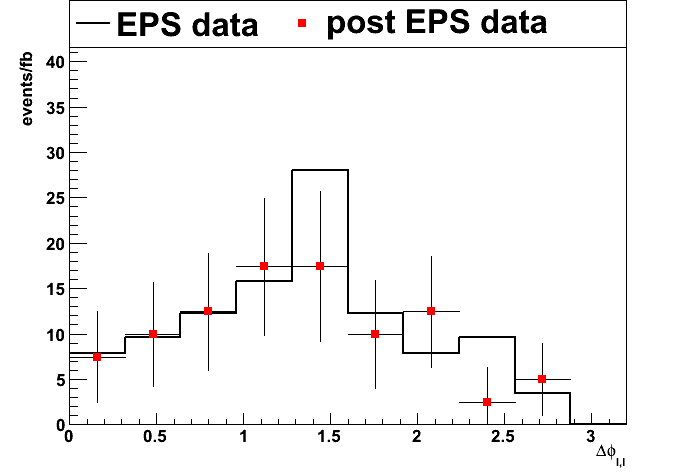
\includegraphics[width=.32\textwidth]{lp_figures/postEPSvalid/hm0/dPhi_ww0jmm.png}}
\subfigure[]{
\centering
\label{subfig:lp_dilepmass_ww0jmm}
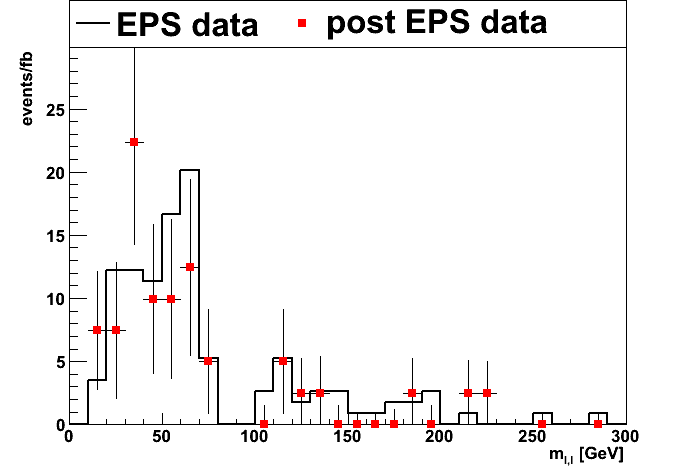
\includegraphics[width=.32\textwidth]{lp_figures/postEPSvalid/hm0/dilepmass_ww0jmm.png}}\\
\subfigure[]{
\centering
\label{subfig:lp_dileppt_ww0jmm}
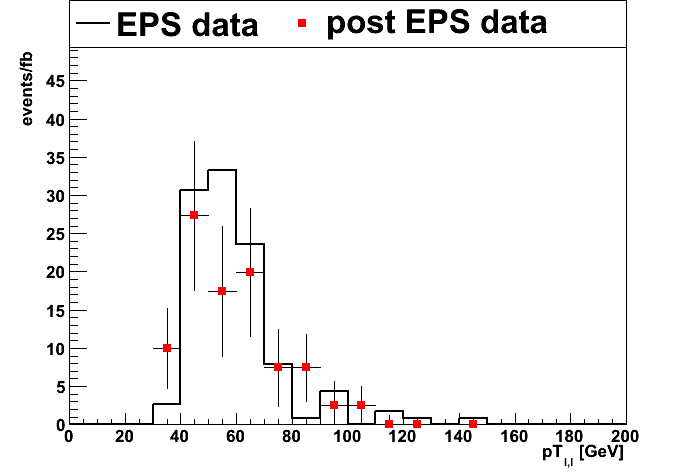
\includegraphics[width=.32\textwidth]{lp_figures/postEPSvalid/hm0/dileppt_ww0jmm.png}}
\subfigure[]{
\centering
\label{subfig:lp_type_ww0jmm}
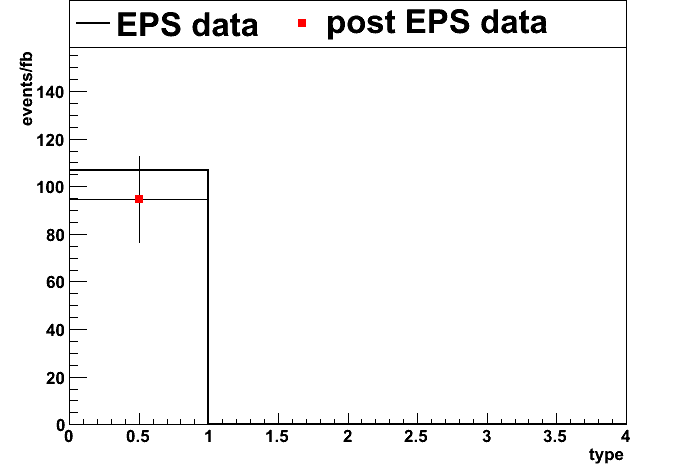
\includegraphics[width=.32\textwidth]{lp_figures/postEPSvalid/hm0/type_ww0jmm.png}}
\caption{EPS and post-EPS data comparison: 0-jet bin, $\mu\mu$ final state. 
\subref{subfig:lp_dPhi_ww0jmm} $\Delta\phi$ between the two leptons;
\subref{subfig:lp_dilepmass_ww0jmm} di-lepton invariant mass;
\subref{subfig:lp_dileppt_ww0jmm} di-lepton transverse momentum;
\subref{subfig:lp_type_ww0jmm} di-lepton type ($\mu\mu$=0, $\mu e$=2, $e\mu$=2, $ee$=3).
}
\label{fig:lp_ww0jmm_dilep}
\end{figure}

\begin{figure}[!hbtp]
\centering
\subfigure[]{
\centering
\label{subfig:lp_lep1pt_ww0jmm}
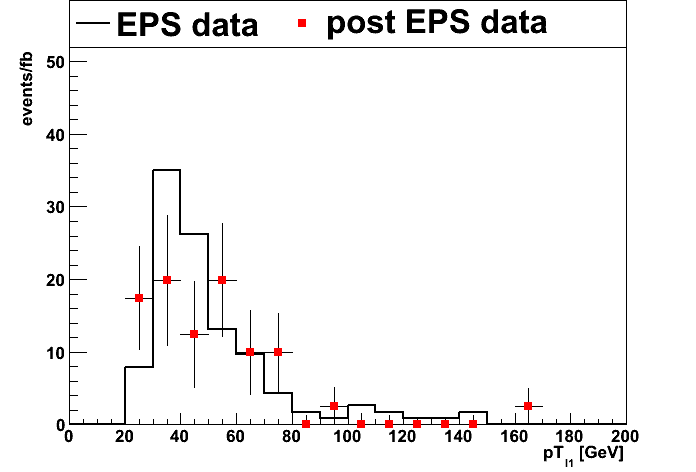
\includegraphics[width=.32\textwidth]{lp_figures/postEPSvalid/hm0/lep1pt_ww0jmm.png}}
\subfigure[]{
\centering
\label{subfig:lp_lep2pt_ww0jmm}
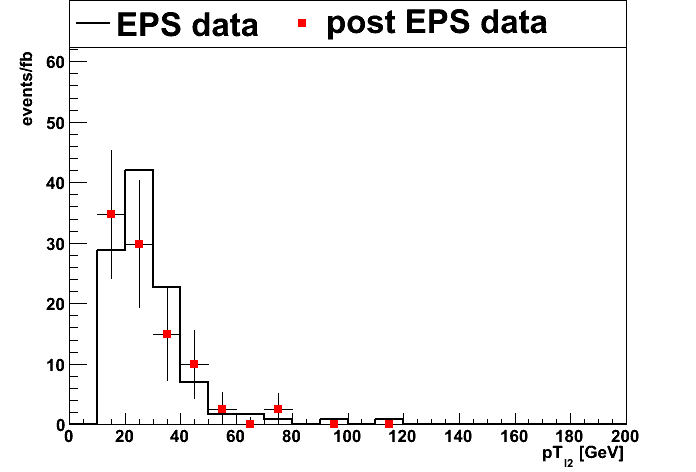
\includegraphics[width=.32\textwidth]{lp_figures/postEPSvalid/hm0/lep2pt_ww0jmm.png}}
\subfigure[]{
\centering
\label{subfig:lp_jet1pt_ww0jmm}
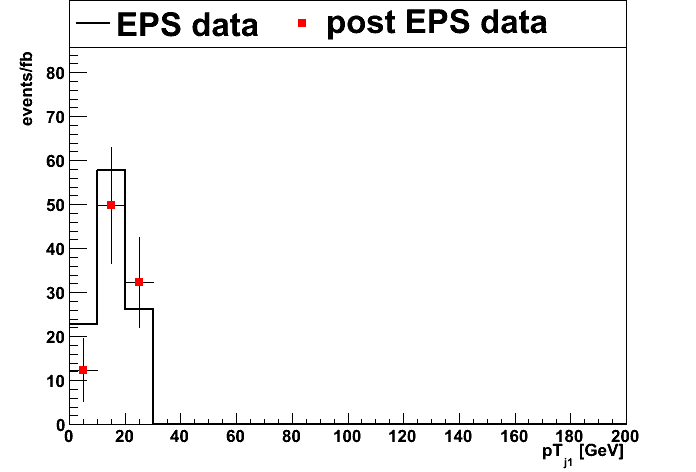
\includegraphics[width=.32\textwidth]{lp_figures/postEPSvalid/hm0/jet1pt_ww0jmm.png}}\\
\subfigure[]{
\centering
\label{subfig:lp_pmet_ww0jmm}
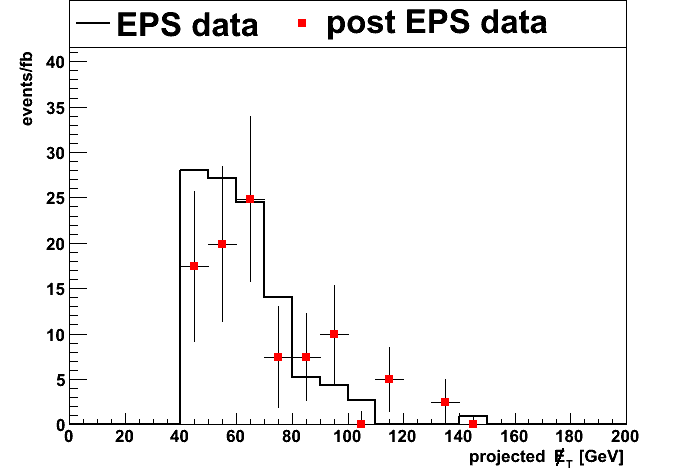
\includegraphics[width=.32\textwidth]{lp_figures/postEPSvalid/hm0/pmet_ww0jmm.png}}
\subfigure[]{
\centering
\label{subfig:lp_pTrackMet_ww0jmm}
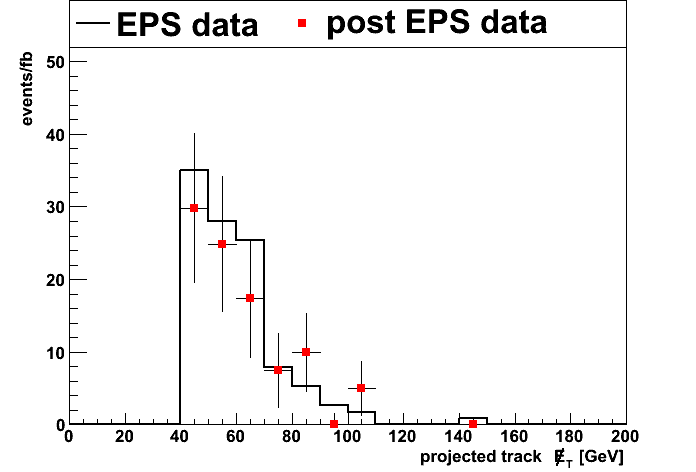
\includegraphics[width=.32\textwidth]{lp_figures/postEPSvalid/hm0/pTrackMet_ww0jmm.png}}
\subfigure[]{
\centering
\label{subfig:lp_mt_ww0jmm}
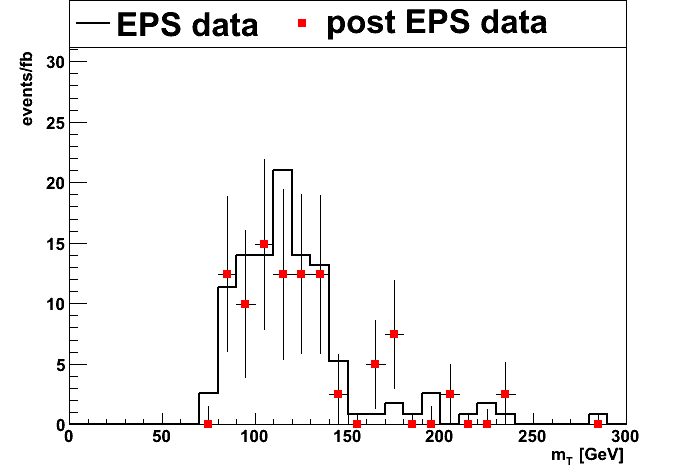
\includegraphics[width=.32\textwidth]{lp_figures/postEPSvalid/hm0/mt_ww0jmm.png}}
\caption{EPS and post-EPS data comparison: 0-jet bin, $\mu\mu$ final state. 
\subref{subfig:lp_lep1pt_ww0jmm} leading lepton $p_T$;
\subref{subfig:lp_lep2pt_ww0jmm} trailing lepton $p_T$;
\subref{subfig:lp_jet1pt_ww0jmm} leading jet $p_T$;
\subref{subfig:lp_pmet_ww0jmm} projected MET;
\subref{subfig:lp_pTrackMet_ww0jmm} projected track-MET;
\subref{subfig:lp_mt_ww0jmm} transverse mass of dilepton-MET system.
}
\label{fig:lp_ww0jmm_lepjetmet}
\end{figure}

\clearpage

\begin{figure}[!hbtp]
\centering
\subfigure[]{
\centering
\label{subfig:lp_dPhi_ww1j}
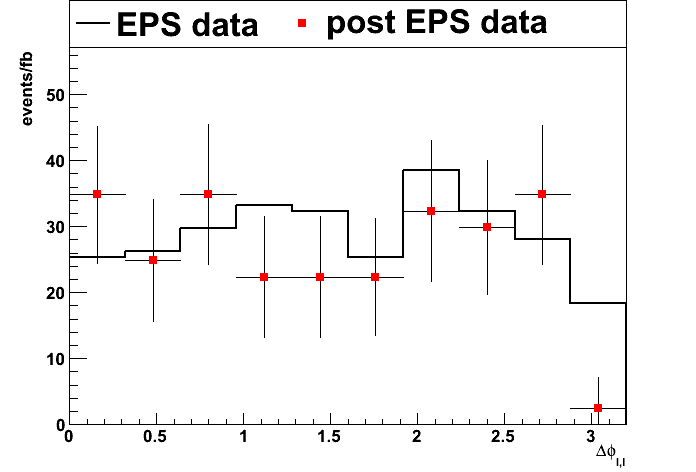
\includegraphics[width=.32\textwidth]{lp_figures/postEPSvalid/hm0/dPhi_ww1j.png}}
\subfigure[]{
\centering
\label{subfig:lp_dilepmass_ww1j}
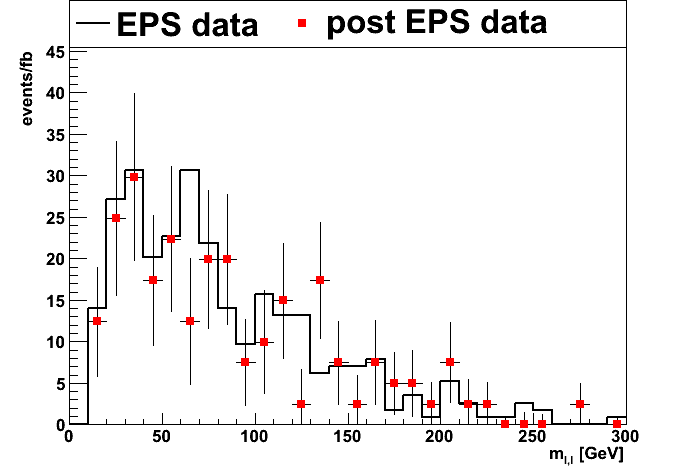
\includegraphics[width=.32\textwidth]{lp_figures/postEPSvalid/hm0/dilepmass_ww1j.png}}\\
\subfigure[]{
\centering
\label{subfig:lp_dileppt_ww1j}
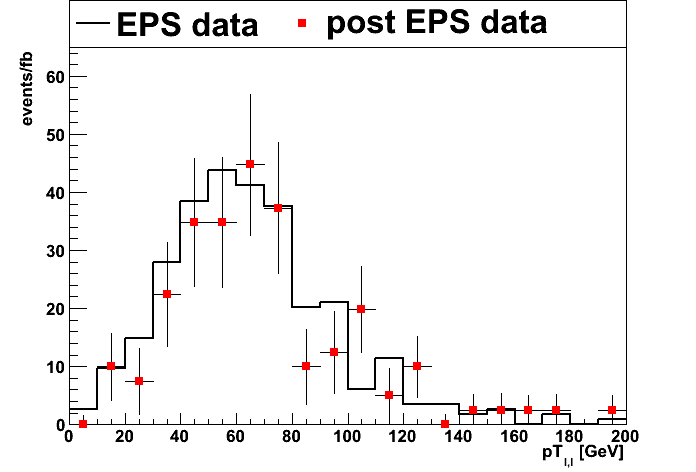
\includegraphics[width=.32\textwidth]{lp_figures/postEPSvalid/hm0/dileppt_ww1j.png}}
\subfigure[]{
\centering
\label{subfig:lp_type_ww1j}
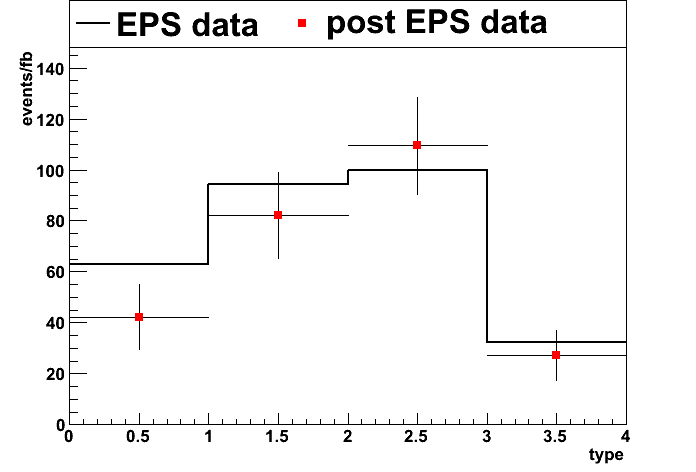
\includegraphics[width=.32\textwidth]{lp_figures/postEPSvalid/hm0/type_ww1j.png}}
\caption{EPS and post-EPS data comparison: 1-jet bin, all final states. 
\subref{subfig:lp_dPhi_ww1j} $\Delta\phi$ between the two leptons;
\subref{subfig:lp_dilepmass_ww1j} di-lepton invariant mass;
\subref{subfig:lp_dileppt_ww1j} di-lepton transverse momentum;
\subref{subfig:lp_type_ww1j} di-lepton type ($\mu\mu$=0, $\mu e$=2, $e\mu$=2, $ee$=3).
}
\label{fig:lp_ww1j_dilep}
\end{figure}

\begin{figure}[!hbtp]
\centering
\subfigure[]{
\centering
\label{subfig:lp_lep1pt_ww1j}
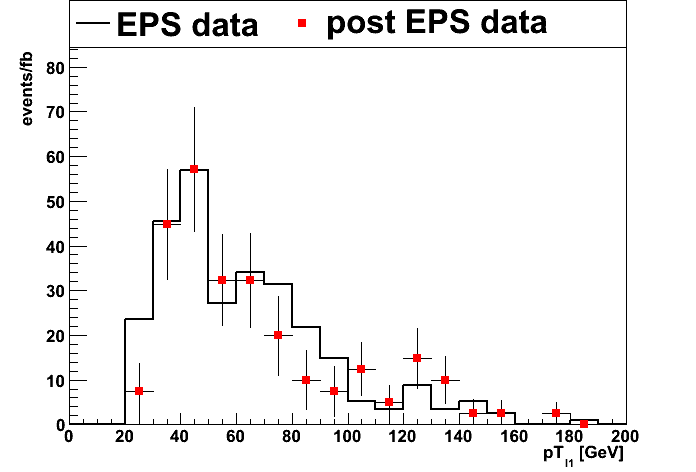
\includegraphics[width=.32\textwidth]{lp_figures/postEPSvalid/hm0/lep1pt_ww1j.png}}
\subfigure[]{
\centering
\label{subfig:lp_lep2pt_ww1j}
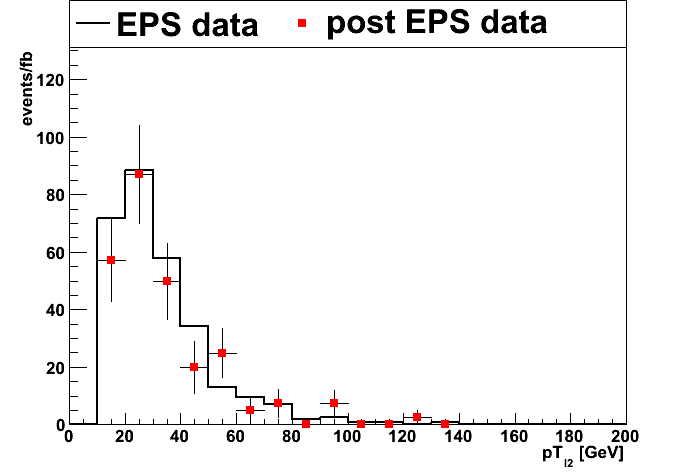
\includegraphics[width=.32\textwidth]{lp_figures/postEPSvalid/hm0/lep2pt_ww1j.png}}
\subfigure[]{
\centering
\label{subfig:lp_jet1pt_ww1j}
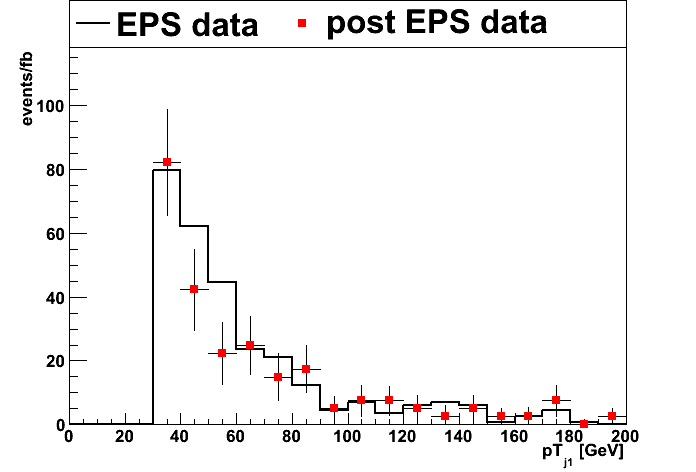
\includegraphics[width=.32\textwidth]{lp_figures/postEPSvalid/hm0/jet1pt_ww1j.png}}\\
\subfigure[]{
\centering
\label{subfig:lp_pmet_ww1j}
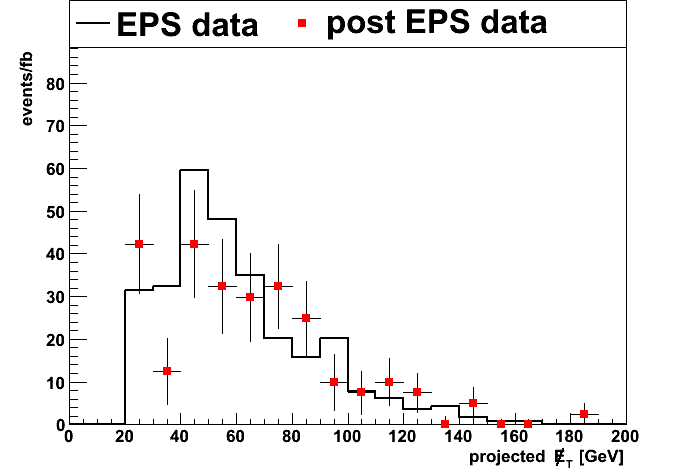
\includegraphics[width=.32\textwidth]{lp_figures/postEPSvalid/hm0/pmet_ww1j.png}}
\subfigure[]{
\centering
\label{subfig:lp_pTrackMet_ww1j}
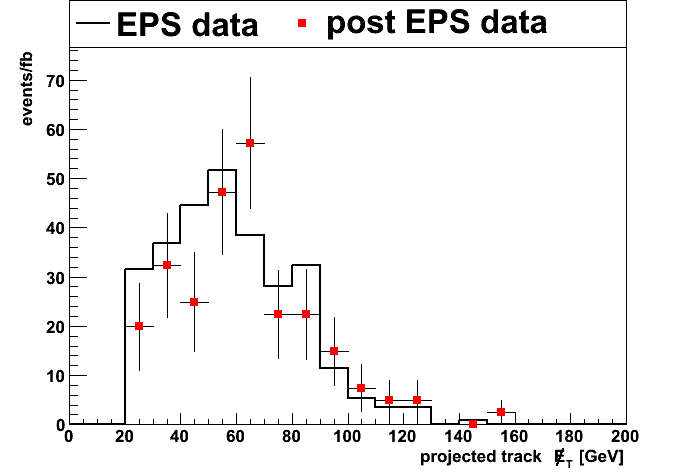
\includegraphics[width=.32\textwidth]{lp_figures/postEPSvalid/hm0/pTrackMet_ww1j.png}}
\subfigure[]{
\centering
\label{subfig:lp_mt_ww1j}
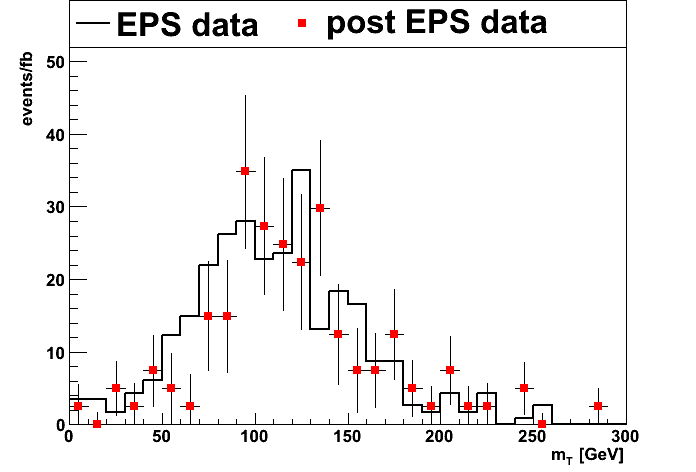
\includegraphics[width=.32\textwidth]{lp_figures/postEPSvalid/hm0/mt_ww1j.png}}
\caption{EPS and post-EPS data comparison: 1-jet bin, all final states. 
\subref{subfig:lp_lep1pt_ww1j} leading lepton $p_T$;
\subref{subfig:lp_lep2pt_ww1j} trailing lepton $p_T$;
\subref{subfig:lp_jet1pt_ww1j} leading jet $p_T$;
\subref{subfig:lp_pmet_ww1j} projected MET;
\subref{subfig:lp_pTrackMet_ww1j} projected track-MET;
\subref{subfig:lp_mt_ww1j} transverse mass of dilepton-MET system.
}
\label{fig:lp_ww1j_lepjetmet}
\end{figure}

\clearpage

\begin{figure}[!hbtp]
\centering
\subfigure[]{
\centering
\label{subfig:lp_dPhi_ww2j}
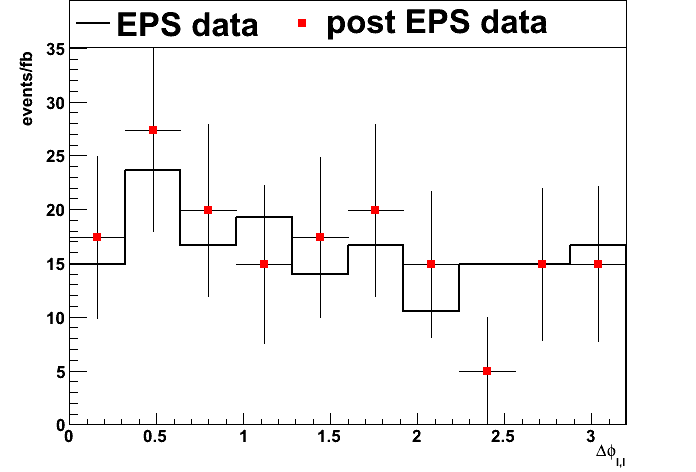
\includegraphics[width=.32\textwidth]{lp_figures/postEPSvalid/hm0/dPhi_ww2j.png}}
\subfigure[]{
\centering
\label{subfig:lp_dilepmass_ww2j}
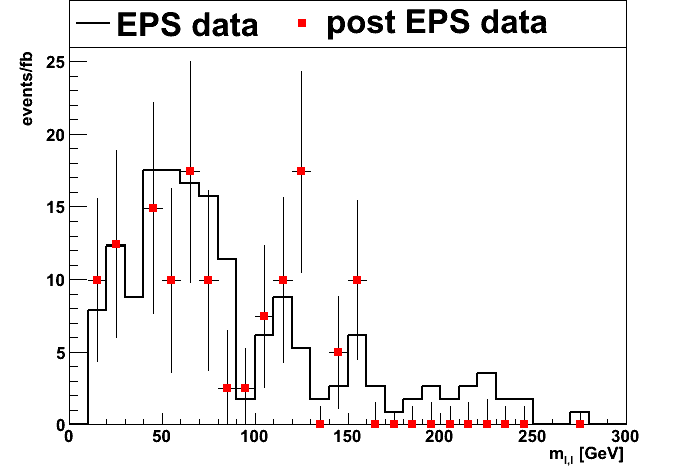
\includegraphics[width=.32\textwidth]{lp_figures/postEPSvalid/hm0/dilepmass_ww2j.png}}\\
\subfigure[]{
\centering
\label{subfig:lp_dileppt_ww2j}
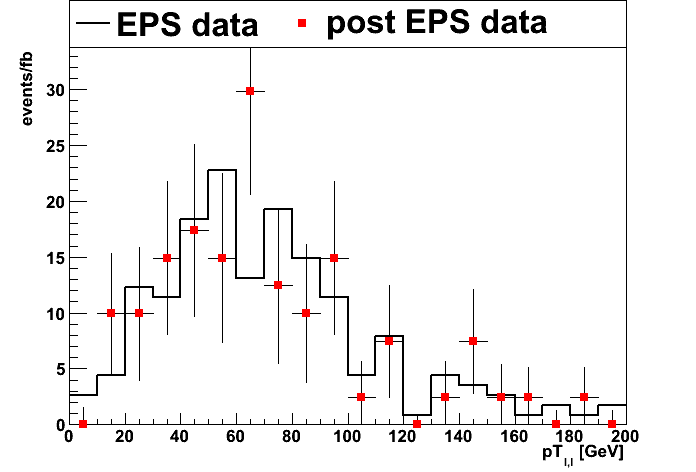
\includegraphics[width=.32\textwidth]{lp_figures/postEPSvalid/hm0/dileppt_ww2j.png}}
\subfigure[]{
\centering
\label{subfig:lp_type_ww2j}
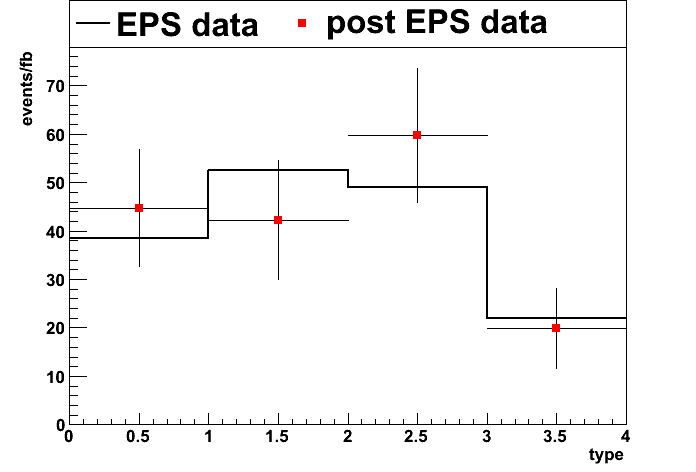
\includegraphics[width=.32\textwidth]{lp_figures/postEPSvalid/hm0/type_ww2j.png}}
\caption{EPS and post-EPS data comparison: 2-jet bin, all final states. 
\subref{subfig:lp_dPhi_ww2j} $\Delta\phi$ between the two leptons;
\subref{subfig:lp_dilepmass_ww2j} di-lepton invariant mass;
\subref{subfig:lp_dileppt_ww2j} di-lepton transverse momentum;
\subref{subfig:lp_type_ww2j} di-lepton type ($\mu\mu$=0, $\mu e$=2, $e\mu$=2, $ee$=3).
}
\label{fig:lp_ww2j_dilep}
\end{figure}

\begin{figure}[!hbtp]
\centering
\subfigure[]{
\centering
\label{subfig:lp_lep1pt_ww2j}
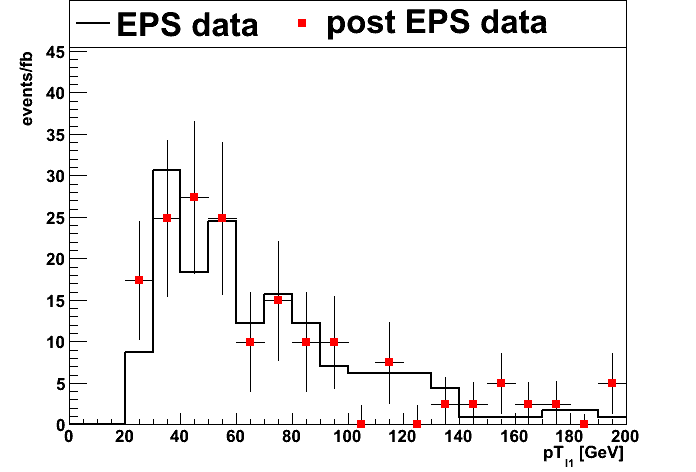
\includegraphics[width=.32\textwidth]{lp_figures/postEPSvalid/hm0/lep1pt_ww2j.png}}
\subfigure[]{
\centering
\label{subfig:lp_lep2pt_ww2j}
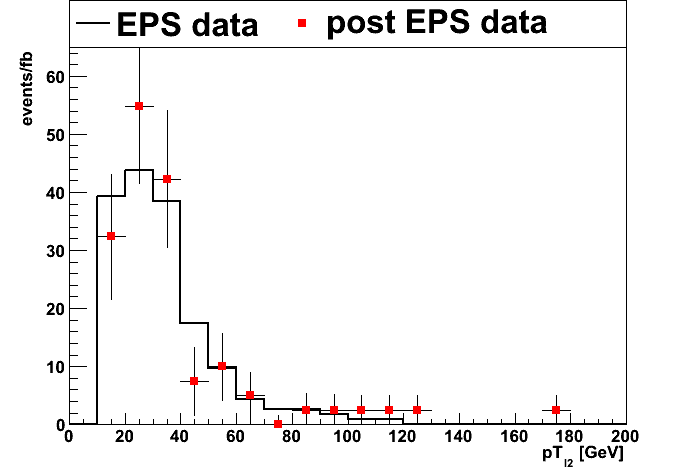
\includegraphics[width=.32\textwidth]{lp_figures/postEPSvalid/hm0/lep2pt_ww2j.png}}
\subfigure[]{
\centering
\label{subfig:lp_jet1pt_ww2j}
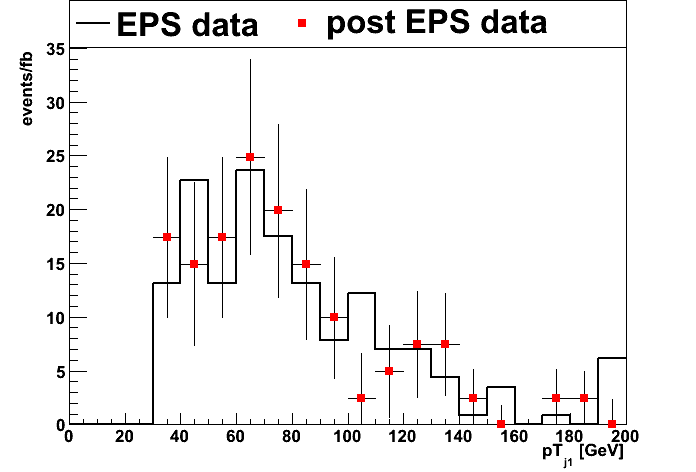
\includegraphics[width=.32\textwidth]{lp_figures/postEPSvalid/hm0/jet1pt_ww2j.png}}\\
\subfigure[]{
\centering
\label{subfig:lp_pmet_ww2j}
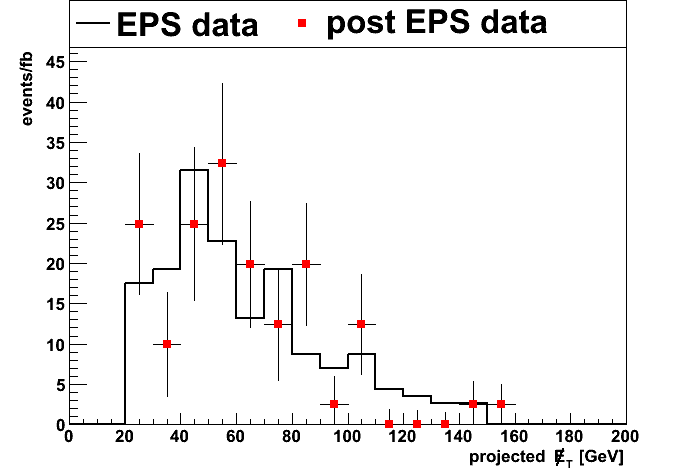
\includegraphics[width=.32\textwidth]{lp_figures/postEPSvalid/hm0/pmet_ww2j.png}}
\subfigure[]{
\centering
\label{subfig:lp_pTrackMet_ww2j}
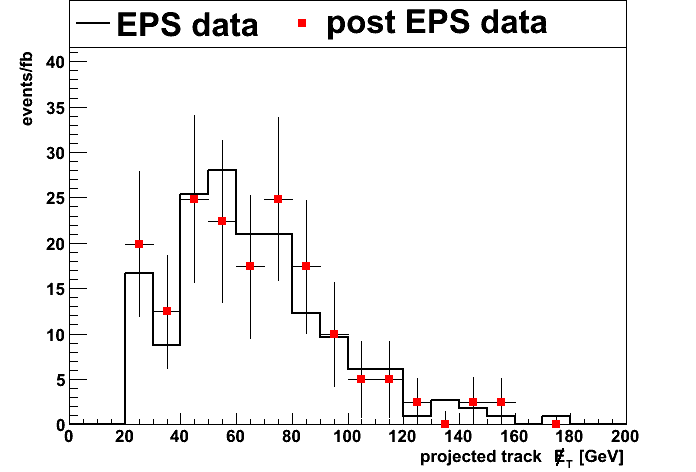
\includegraphics[width=.32\textwidth]{lp_figures/postEPSvalid/hm0/pTrackMet_ww2j.png}}
\subfigure[]{
\centering
\label{subfig:lp_mt_ww2j}
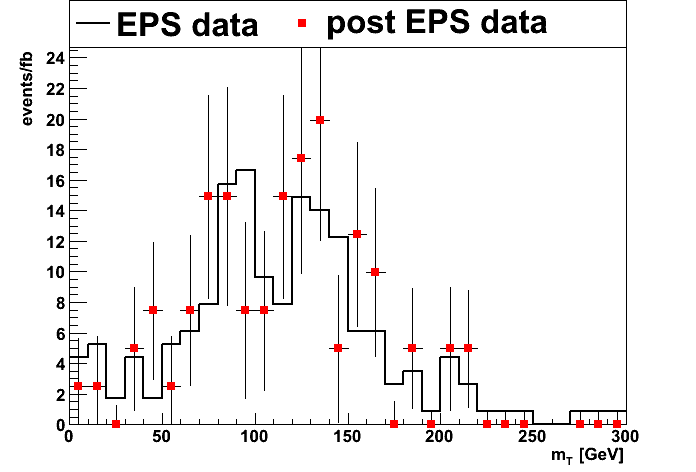
\includegraphics[width=.32\textwidth]{lp_figures/postEPSvalid/hm0/mt_ww2j.png}}
\caption{EPS and post-EPS data comparison: 2-jet bin, all final states. 
\subref{subfig:lp_lep1pt_ww2j} leading lepton $p_T$;
\subref{subfig:lp_lep2pt_ww2j} trailing lepton $p_T$;
\subref{subfig:lp_jet1pt_ww2j} leading jet $p_T$;
\subref{subfig:lp_pmet_ww2j} projected MET;
\subref{subfig:lp_pTrackMet_ww2j} projected track-MET;
\subref{subfig:lp_mt_ww2j} transverse mass of dilepton-MET system.
}
\label{fig:lp_ww2j_lepjetmet}
\end{figure}

\clearpage
